\documentclass[sigplan, review]{acmart}

\usepackage{booktabs} % For formal tables
\usepackage{xspace} 


% Copyright
\setcopyright{none}
%\setcopyright{acmcopyright}
%\setcopyright{acmlicensed}
%\setcopyright{rightsretained}
%\setcopyright{usgov}
%\setcopyright{usgovmixed}
%\setcopyright{cagov}
%\setcopyright{cagovmixed}

\settopmatter{printacmref=false}

% DOI
\acmDOI{}

% ISBN
\acmISBN{}

%Conference
\acmConference[SC'18]{Supercomputing Conference}{November 2018}{Dallas,TX USA}
\acmYear{}
\copyrightyear{2018}

%\acmPrice{15.00}

%\acmBadgeL[http://ctuning.org/ae/ppopp2016.html]{ae-logo}
%\acmBadgeR[http://ctuning.org/ae/ppopp2016.html]{ae-logo}

% Submission ID
%\acmSubmissionID{123-A56-BU3}

\newcommand{\RAC}{RAC\xspace}
\newcommand{\RACfull}{Recursive Algebraic Coloring\xspace}
\newcommand{\RACE}{RACE\xspace}
\newcommand{\RACEfull}{Recursive Algebraic Coloring Engine\xspace}
\newcommand{\DONE}{distance-$1$\xspace}
\newcommand{\DTWO}{distance-$2$\xspace}
\newcommand{\DK}{distance-$k$\xspace}
\newcommand{\etal}{et al.\xspace}
\newcommand{\RSB}{RSB\xspace}
\newcommand{\SpMV}{SpMV\xspace}
\newcommand{\SymmSpmv}{SymmSpMV\xspace}
\newcommand{\SpMTV}{SpMTV\xspace}
\newcommand{\GS}{GS\xspace}
\newcommand{\SYMMGS}{SymmGS\xspace}
\newcommand{\KACZ}{KACZ\xspace}
\newcommand{\SYMMKACZ}{SymmKACZ\xspace}
\newcommand{\Intel}{Intel\xspace}
\newcommand{\AMD}{AMD\xspace} 
\newcommand{\IVB}{Ivy-Bridge\xspace}
\newcommand{\BDW}{Broadwell\xspace}
\newcommand{\SKX}{Sky-Lake\xspace}
\newcommand{\NAP}{Naples\xspace}
\newcommand{\EPY}{Epyc\xspace}
\newcommand{\CRS}{CRS\xspace}
\newcommand{\CRSfull}{Compressed Row Storage\xspace}
\newcommand{\MC}{MC\xspace}
\newcommand{\MCfull}{multi-coloring\xspace}
\newcommand{\ABMC}{ABMC\xspace}
\newcommand{\ABMCfull}{algebraic block multi-coloring\xspace}
\newcommand{\NNZR}{$N_{nzr}$\xspace}
\newcommand{\NNZRSYMM}{$N_{nzr}^{symm}$\xspace}
\newcommand{\NNZRmath}{N_{nzr}\xspace}
\newcommand{\NNZRmathSYMM}{N_{nzr}^{symm}\xspace}
\newcommand{\LIKWID}{LIKWID\xspace}
\newcommand{\likwidBench}{$likwid-bench$\xspace}
\newcommand{\LLC}{LLC\xspace}
\newcommand{\LLCfull}{last level cache\xspace}
\newcommand{\ie}{i.e.,\xspace}
\newcommand{\ESSEX}{ESSEX\xspace}
\newcommand{\LCCfull}{Low Core Count\xspace}
\newcommand{\LCC}{LCC\xspace}
\newcommand{\HCCfull}{High Core Count\xspace}
\newcommand{\HCC}{HCC\xspace}
\newcommand{\MB}{MB\xspace}
\newcommand{\KB}{kB\xspace}
\newcommand{\GB}{GB\xspace}
\newcommand{\TB}{TB\xspace}
\newcommand{\SIMD}{SIMD\xspace}
\newcommand{\RCMfull}{Reverse Cuthill McKee\xspace}
\newcommand{\RCM}{RCM\xspace}
\newcommand{\CMfull}{Cuthill McKee\xspace}
\newcommand{\BFSfull}{Breadth First Search\xspace}
\newcommand{\BFS}{BFS\xspace}
\newcommand{\CPU}{CPU\xspace}
\newcommand{\pt}{pt.\xspace}
\newcommand{\STEX}{2d-7pt stencil\xspace}
\newcommand{\Inorder}{In order\xspace}
\newcommand{\inorder}{in order\xspace}
\newcommand{\levelPtr}{{\tt level\_ptr}\xspace}
\newcommand{\atleast}{at least\xspace}
\newcommand{\totalLvl}{$n_l$\xspace}
\newcommand{\totalLvlMATH}{n_l}
\newcommand{\level}{$level$\xspace}
\newcommand{\levels}{$levels$\xspace}
\newcommand{\levelGroup}{$level \text{  } group$\xspace}
\newcommand{\levelGroups}{$level \text{  } groups$\xspace}
\newcommand{\LevelGroups}{$Level \text{  } groups$\xspace}
\newcommand{\eg}{e.g.,\xspace}
\newcommand{\aka}{a.k.a.\xspace}
\newcommand{\subgraph}{sub-graph\xspace}
\newcommand{\subgraphs}{sub-graphs\xspace}
\newcommand{\levelTree}{{\tt level\_tree}\xspace}
\newcommand{\HPC}{HPC\xspace}
\newcommand{\effPar}{\emph{effective parallelism}\xspace}
\newcommand{\effRow}{\emph{effective row}\xspace}
\newcommand{\EffRow}{\emph{Effective row}\xspace}
\newcommand{\nthreads}{${n_{t}}$\xspace}
\newcommand{\nthreadsMath}{n_{t}\xspace}
\newcommand{\nrows}{${n_{r}}$\xspace}
\newcommand{\nrowsMath}{n_{r}\xspace}
\newcommand{\nrowsNospace}{${n_{r}}$}
\newcommand{\nnz}{${n_{nz}}$\xspace}
\newcommand{\nnzMath}{n_{nz}\xspace}
\newcommand{\nrowsEff}{${n_{r}^{eff}}$\xspace}
\newcommand{\nrowsEffMath}{n_{r}^{eff}\xspace}
\newcommand{\threadEff}{${n_{t}^{eff}}$\xspace}
\newcommand{\threadEffMath}{n_{t}^{eff}\xspace}
\newcommand{\upto}{up to \xspace}
\newcommand{\fracUnit}[2]{\Big[\frac{\mbox{#1}}{\mbox{#2}}\Big]}
\newcommand{\unit}[1]{\Big[\mbox{#1}\Big]}
\newcommand{\roofline}{roofline\xspace}
\newcommand{\METIS}{METIS\xspace}
\newcommand{\COLPACK}{COLPACK\xspace}
\newcommand{\SPMP}{Intel SpMP\xspace}
\newcommand{\MKL}{MKL\xspace}

\begin{document}
\title[RACE]{Recursive Algebraic Coloring Engine}
%\titlenote{Produces the permission block, and
%  copyright information}
\subtitle{Poster Summary}
%\subtitlenote{The full version of the author's guide is available as
%  \texttt{acmart.pdf} document}

\author{Christie Louis Alappat}
%\orcid{1234-5678-9012-3456}
\affiliation{%
	\institution{Friedrich-Alexander-Universit{\"a}t Erlangen-N{\"u}rnberg}
	\city{Erlangen}
	\country{Germany}}
\email{christie.alappat@fau.de}

\author{Georg Hager}
\affiliation{%
	\institution{Friedrich-Alexander-Universit{\"a}t Erlangen-N{\"u}rnberg}
	\city{Erlangen}
	\country{Germany}
}
\email{georg.hager@fau.de}

\author{Gerhard Wellein}
\affiliation{%
	\institution{Friedrich-Alexander-Universit{\"a}t Erlangen-N{\"u}rnberg}
	\city{Erlangen}
	\country{Germany}
}
\email{gerhard.wellein@fau.de}

\author{Olaf Schenk}
\affiliation{%
	\institution{Institute of Computational Science}
	\city{Lugano}
	\country{Switzerland}
}
\email{olaf.schenk@usi.ch}

% The default list of authors is too long for headers.
\renewcommand{\shortauthors}{C. Alappat et al.}



\begin{abstract}
Many iterative numerical methods for sparse systems and important building blocks of sparse linear algebra feature strong data dependencies. They may be loop-carried dependencies as they occur in many iterative solvers or preconditioners (e.g., Gauss-Seidel, Kaczmarz) or write conflicts as in the parallelization of building blocks such as symmetric sparse matrix vector or sparse matrix transpose vector multiplication. Scalable, hardware-efficient parallelization of such kernels is known to be a challenge. Most of the typical solutions suffer from low performance on modern hardware, are highly matrix specific, or require tailored matrix storage formats.

In this poster we show a novel method called Recursive Algebraic Coloring (RAC), which achieves high hardware efficiency on modern multi-core architectures and works with simple data formats like compressed row storage (CRS). RAC uses a recursive level-based method that aims at finding optimal permutations while preserving data locality. It is implemented and consolidated into a user-friendly library called Recursive Algebraic Coloring Engine (RACE). A thorough performance analysis shows that RACE outperforms traditional Multicoloring methods and Intel MKL implementations with a factor of 2--2.5$\times$. We are on par with Algebraic Block Multicoloring (ABMC) for small matrices, while for large matrices we gain almost a factor of 1.5--2$\times$.
\end{abstract}



\keywords{Shared memory parallel, Distance-k dependency, Graph algorithm, Sparse matrices, Sparse linear algebra, Performance}

%\begin{teaserfigure}
%  \includegraphics[width=\textwidth]{sampleteaser}
%  \caption{This is a teaser}
%  \label{fig:teaser}
%\end{teaserfigure}


\maketitle

	
\section{Problem \& Motivation}
	Sparse linear algebra is a key component in many of the scientific simulations
	ranging from quantum physics to fluid and structural mechanics.
	But unfortunately many iterative numerical methods for sparse systems 
	and important building 	blocks of sparse linear algebra feature strong 
	data dependencies rendering them difficult to be parallelized.
	They may be	loop-carried dependencies as they occur in
	many iterative solvers or preconditioners (e.g., Gauss-Seidel, Kaczmarz) 
	or write conflicts as in the parallelization of building blocks such 
	as symmetric sparse matrix vector or sparse matrix transpose vector multiplication.
	Scalable, hardware-efficient parallelization of such kernels is known to be a 
	challenge. Most of the typical solutions suffer from low performance
	on modern hardware, are highly matrix specific, or require tailored
    matrix storage formats.

	In this paper we present a novel approach called \acrshort{RACE} that helps in
	solving the general distance-k dependency problem for sparse kernels in a
	hardware efficient manner. The \acrshort{RACE} method is motivated by the
	shortcomings of multicoloring methods that are frequently used in this scenario.
	The method works on simple data storage formats
	like \acrfull{CRS}, and is highly scalable to meet the requirements of 
	modern CPU based compute nodes. \medskip

\noindent\textbf{Outline}


\noindent	The paper is structured as follows. In \cref{sec:background} we discuss
	the commonly occurring dependency problems and the conventional
	approaches used to solve such kind of dependencies. \Cref{sec:uniqueness} 
	shows the general issues that occur while using these conventional
	approaches. We then describe the \acrshort{RACE} method, it's uniqueness
	and how its	basic design circumvents the commonly occurring problems. 
	Towards the end	in \cref{sec:results} we show the performance advantage
	of \acrshort{RACE} compared to others and apply the method to implement
	a parallel iterative sparse eigen value solver called FEAST, which we 
	believe is the first iterative implementation of this eigen value solver.
	
	\begin{comment}
	In this paper we present a novel approach called \acrshort{RACE} that helps in
	solving the general distance-k dependency problem for sparse kernels in a
	hardware efficient manner. The \acrshort{RACE} method is motivated by the
	shortcomings of multicoloring methods that are frequently used in this scenario.
	The method uses a recursive level-based approach to find optimal permutations
	while preserving good data locality. A thorough performance analysis shows that
	our method achieves high hardware efficiency on modern multi-core architectures
	and it outperforms traditional \acrfull{MC} and \acrshort{MKL} implementations
	by a factor of 2--2.5$\times$. We are on par with \acrfull{ABMC} method for
	small matrices, while for large matrices we gain almost a factor of
	1.5--2$\times$. Owing to the success of parallel implementations of
	sparse kernels having dependencies we further demonstrate first results
	of parallel iterative FEAST eigen solver using CGMN internal solver.
	\end{comment}


\section{Background \& Related Work} \label{sec:background}
Many kernels that come across in sparse linear algebra are hard to 
be parallelized due to dependencies. 
%The two main class of dependencies that occur in this field are \DONE
%dependency as in Gauss-Seidel iteration or a \DTWO dependency as they 
%occur in \acrfull{KACZ} or \acrfull{SymmSpMV}. 

\begin{algorithm}[tb]
	\caption{\label{alg:symmSpMV} \acrshort{SymmSpMV} kernel,  $b=Ax$, in \acrshort{CRS} format.}
	\begin{algorithmic}[1]
		\For{$row=1:nrows$}
			\State{$diag\_idx=rowPtr[row]$}
			\State{$b[row] += A[diag\_idx]*x[row]$}
			\For{$idx=rowPtr[row]+1:rowPtr[row+1]$}
				\State{$b[row] += A[idx]*x[col[idx]]$}
				\State{$b[col[idx]] += A[idx]*x[row]$} 
			\EndFor
		\EndFor
	\end{algorithmic}
\end{algorithm}

One such example is \acrfull{SymmSpMV}. \Cref{alg:symmSpMV} shows
the pseudo-code of \acrshort{SymmSpMV} kernel in \acrshort{CRS} matrix storage
format. The kernel exploits the symmetry of the matrix ($A_{ij} = A_{ji}$) to
reduce storage size and overall memory traffic. 
However \acrshort{SymmSpMV} cannot be parallelized straightforward.
For instance if two different threads work on
two different rows in parallel it could potentially lead to simultaneous 
writing to the same element ($b[col[idx]]$) of the indirectly accessed $b$ vector.
This leads to write conflicts, and such kinds of dependency is called a \DTWO
dependency. Such dependency along with \DONE as in Gauss-Seidel iteration
are the commonly occurring dependencies in sparse kernels. In this paper
we concentrate on \DTWO dependency problems, although the underlying method and
library is capable of handling general \DK dependencies.


Many solutions to these dependency problems have been proposed, such as 
locking method and thread-private target arrays \cite{sparseX,thread_private_symm_spmv}.
But these approaches could lead to performance degradation depending
on the matrix due to serialization or increase in data traffic respectively.
Recent researches include in the direction of special storage formats like
 CSB \cite{CSB} or RSB \cite{RSB} but this require rewriting of existing 
 code and lot of tuning. Another popular approach in the field is matrix 
reordering technique, on which we focus here.
One of the earliest work on reordering is the red-black 
Gauss--Seidel scheme~\cite{RBGS}. 
Later it has been generalized for sparse matrices and \DK dependent 
problems by well-known \acrfull{MC} approaches \cite{MC, COLPACK}. 
Variants like \acrfull{ABMC} \cite{ABMC} have tried to
improve the  performance of the \acrshort{MC} methods. In \cite{feast_mc},
\acrshort{MC} was applied to \acrshort{KACZ} kernel having  \DTWO dependency. 

\section{Uniqueness of the approach} \label{sec:uniqueness}
Approaches like \acrshort{MC} can help in parallelization of the kernel, however
the method can destroy data locality of the matrix leading to low performance.
\setlength{\belowcaptionskip}{-12pt}
\begin{figure}[tb]
	 \subfloat[Scaling performance]{\label{fig:motivation_symm_spmv}\scalebox{0.8}{\documentclass{standalone}
\usepackage{tikz}
\usepackage{pgfplots}
\pgfplotsset{width=9cm,height=12cm,compat=1.3}
\usepackage{filecontents}
\usetikzlibrary{patterns}
\usepackage{pgfplotstable}

\def\matrixFile{../data_skx}
\def\matrix{Spin-26}
%\def\matrixFileNowait{../data/motivation_nowait/Spin-26}
%\def\matrixFileMKL{../data/motivation_mkl/Spin-26}
\def\matrixName{Spin-26 }

\definecolor{color1}{RGB}{230,97,1}
\definecolor{color2}{RGB}{253,184,99}
\definecolor{color3}{RGB}{178,171,210}
\definecolor{color4}{RGB}{94,60,153}

\begin{document}
	\pgfplotstableread[col sep=comma] {\matrixFile/MKL/\matrix/spmv.txt} \SPMV
	\pgfplotstableread[col sep=comma] {\matrixFile/MC_RCM/\matrix/symm_spmv.txt} \SYMMSPMVMC
	\pgfplotstableread[col sep=comma] {\matrixFile/ABMC_RCM/\matrix/symm_spmv.txt} \SYMMSPMVABMC
	\pgfplotstableread[col sep=comma] {\matrixFile/RACE/\matrix/symm_spmv.txt} \SYMMSPMVRACE
	\pgfplotstableread[col sep=space] {\matrixFile/nnz} \NNZfile
		
	\pgfplotstablegetelem{0}{nnz}\of\NNZfile
	\pgfmathsetmacro{\NNZ}{\pgfplotsretval}
		
	
\centering
\begin{tikzpicture}


  \def\xmin{0}
  \def\xmax{10}
  \def\ymin{0}
  \def\ymax{30}
 
  \begin{axis}[ xlabel={\huge{$N_t$}}, ylabel={\huge{Performance (GF/s)}}, ymode=linear,
x tick label style={font={\huge}},
y tick label style={font={\huge}},
xtick={0,4,8,12,16,20},
%xtick={1000, 2744, 5832, 10648, 17576, 27000, 39304, 54872, 74088},
%xticklabels={$10^3$, %$14^3$
%  , $18^3$, $22^3$, $26^3$, $30^3$, $34^3$, $38^3$, $42^3$},
scaled ticks=false,
%xmode=log,
xmin=0,xmax = 20,
ymin=0,ymax=17.5,
%ymin=0, ymax=14,
legend style={legend pos=north west, font=\LARGE}]

   \addplot+[line width=2, color=color1, mark options={color1}, mark=diamond*,] table[x =THREAD,y =PERF (GFlop/s),col sep=comma] {\SPMV}; \label{plot_one}
   \addlegendentry{SpMV}

   \addplot+[line width=2, color=color3, mark options={color3},  mark=square*,] table[x =THREAD,y =PERF (GFlop/s),col sep=comma] {\SYMMSPMVMC}; \label{plot_two}
  \addlegendentry{SymmSpMV MC}

   \addplot+[line width=2, color=color4, mark options={color4}, mark=triangle*] table[x =THREAD,y =PERF (GFlop/s),col sep=comma] {\SYMMSPMVABMC}; \label{plot_three}
   \addlegendentry{SymmSpMV ABMC}
   
%   \addplot+[line width=2, color=orange, mark options={orange}] table[x =THREAD,y =PERF (GFlop/s),col sep=comma] {\SYMMSPMVRACE}; \label{plot_four}
%   \addlegendentry{SymmSpMV RAC}
   
   
 \end{axis}

\end{tikzpicture}

\end{document}
}}\hspace{1em}
	 \subfloat[Data traffic]{\label{fig:motivation_data}\scalebox{0.8}{\pgfplotsset{width=5cm,height=7cm,compat=1.3}
\def\matrixFile{pics/Spin-26/data}
\def\matrix{Spin-26}
\def\matrixName{Spin-26 }
\newcommand{\ideal}{11.25}

%\begin{document}
	\pgfplotstableread[col sep=comma] {\matrixFile/MKL/\matrix/spmv.txt} \SPMV
	\pgfplotstableread[col sep=comma] {\matrixFile/MC_RCM/\matrix/spmv.txt} \SPMVMC
	\pgfplotstableread[col sep=comma] {\matrixFile/MC_RCM/\matrix/symm_spmv.txt} \SYMMSPMVMC
	\pgfplotstableread[col sep=comma] {\matrixFile/ABMC_RCM/\matrix/spmv.txt} \SPMVABMC
	\pgfplotstableread[col sep=comma] {\matrixFile/ABMC_RCM/\matrix/symm_spmv.txt} \SYMMSPMVABMC
	\pgfplotstableread[col sep=comma] {\matrixFile/RACE/\matrix/symm_spmv.txt} \SYMMSPMVRACE
	\pgfplotstableread[col sep=space] {\matrixFile/nnz} \NNZfile
		
	\pgfplotstablegetelem{0}{nnz}\of\NNZfile
	\pgfmathsetmacro{\NNZ}{\pgfplotsretval}
		
	
		\begin{tikzpicture}[tight background,trim axis left]
		\begin{axis}[
	%	width  = 12cm,
%		height = 11cm,
		major x tick style = transparent,
		minor ytick={1, 5, 10, 15, 20, 25, 30 ,35,40},
		grid = minor,
		ybar=2*\pgflinewidth,
		bar width=16pt,
		ymajorgrids = true,
		grid style={dashed, gray!40},
		ylabel = {B/$N_{NZ}$},
		symbolic x coords={SpMV, MC, ABMC},
		x tick label style={rotate=25,font={\large}},
		y tick label style={font={\Large}},
		xtick = data,
		scaled y ticks = false,
		enlarge x limits=0.25,
		ymin=0,% ymax=42,
		ymax=58,
		legend cell align=left,
		legend style={
			%at={(1,1.05)},
			%anchor=south east,
			%column sep=1ex,
			legend pos=north west
		},
		]
		

		\pgfkeys{/pgf/fpu}

		\pgfplotstablegetelem{9}{MEM (GB)}\of\SPMV
		\pgfmathsetmacro{\memSPMV}{\pgfplotsretval*1*1/(\NNZ*0.5*1e-8)} %change to SpMV
		\pgfplotstablegetelem{9}{MEM (GB)}\of\SPMVMC
		\pgfmathsetmacro{\memSPMVMC}{\pgfplotsretval*1*1/(\NNZ*0.5*1e-8)}
		\pgfplotstablegetelem{9}{MEM (GB)}\of\SPMVABMC
		\pgfmathsetmacro{\memSPMVABMC}{\pgfplotsretval*1*1/(\NNZ*0.5*1e-8)}
		\pgfplotstablegetelem{9}{MEM (GB)}\of\SYMMSPMVMC
		\pgfmathsetmacro{\memSYMMSPMVMC}{\pgfplotsretval*1*1/(\NNZ*0.5*1e-8)}
		\pgfplotstablegetelem{9}{MEM (GB)}\of\SYMMSPMVABMC
		\pgfmathsetmacro{\memSYMMSPMVABMC}{\pgfplotsretval*1*1/(\NNZ*0.5*1e-8)}
		\pgfplotstablegetelem{9}{MEM (GB)}\of\SYMMSPMVRACE
		\pgfmathsetmacro{\memSYMMSPMVRACE}{\pgfplotsretval*1*1/(\NNZ*0.5*1e-8)}
		
		\addplot[pattern=horizontal lines]%[fill=gray!60!black]%style={ppurple,fill=ppurple}]
		coordinates {(SpMV,\memSPMV) (MC,\memSYMMSPMVMC) (ABMC,\memSYMMSPMVABMC)};
			
		\pgfkeys{/pgf/fpu=false}

		\addplot[draw=red,smooth,dashed, line width=2pt] coordinates { (MC,\ideal) (ABMC,\ideal)};
				
		\legend{MEM traffic, Ideal SymmSpMV}
		
		\addplot[draw=red,smooth,dashed, line width=2pt, shorten >=-1em, shorten <=-4em] coordinates { (MC,\ideal) (ABMC,\ideal)};
		\end{axis}
	%	\node at (6.5,10) {Data traffic Comparison using LIKWID};
		\end{tikzpicture}
%\end{document}
}}
	\caption{\label{fig:motivation}(a) Performance of \acrshort{SymmSpMV} with 
		\acrshort{MC} and \acrshort{ABMC} compared to \acrshort{SpMV}. 
		(b) Average main memory data traffic in bytes (B) per nonzero entry ($\acrshort{nnz}$) 
		of the full matrix as measured with \LIKWID tool \cite{LIKWID}.}
\end{figure}
To demonstrate the effect we present in \cref{fig:motivation} performance and 
data transfer volumes of  \acrshort{SymmSpMV} operation on \texttt{Spin-26} matrix 
taken from quantum physics application. \Cref{fig:motivation_symm_spmv}
shows performance in gigaflops (\GF) as a function of thread (core) count 
on a single chip (1 socket) of \Intel \IVB (E5-2660) architecture 
clocked at 2.2\GHZ.
The general variant  of sparse matrix-vector multiplication (\acrshort{SpMV})
 using the full matrix  serves as the yardstick for comparison. 
Based on a naive performance analysis, as most of the sparse
kernels are highly memory bound on modern architectures
one would expect \acrshort{SymmSpMV} performance 
to be almost twice that of \acrshort{SpMV}, due to half the data traffic. 
However the \acrshort{SymmSpMV} implementation using \acrshort{MC} is more
than three times slower.

 The reason for this is the nature of \acrlong{MC} 
permutation (reordering). For \DTWO coloring, \acrshort{MC}
groups rows that do not overlap in any column entries \cite{dist_k_def} 
(structurally orthogonal rows). These group of rows are referred to as
a color. Due to this grouping one can parallelize all the rows within a color, 
as this ensures in our \acrshort{SymmSpMV} example (see \cref{alg:symmSpMV})
that threads operate on different rows having entirely different 
$col[idx]$ avoiding write conflicts in $b$ vector.

\begin{figure}[b]
	\centering
	\subfloat[Original ordering]{\scalebox{0.625}{%\documentclass{standalone}
%\usepackage{tikz}

%\begin{document}

%\begin{minipage}{0.55\textwidth}
%	\centering
	\def\rowperm{{0, 1, 2, 3, 4, 5, 6}}
	%\def\colperm{{0, 1, 2, 3, 4, 5, 6}}
	\def\colperm{{0, 1, 2, 3, 4, 5, 6}}
	\scalebox{0.7}{\begin{tikzpicture}
		\foreach \x in {0,1}
		\fill[gray] (\colperm[\x]-1,6) rectangle (\colperm[\x],7);
		\foreach \y in {0,1,2,3,4}  
			\foreach \x in {0,1,2}
				\fill[gray] (\colperm[\x]-1+\y,5-\y) rectangle (\colperm[\x]+\y,6-\y);   
		\foreach \x in {0,1}
			\fill[gray] (\colperm[5+\x]-1,0) rectangle (\colperm[5+\x],1); 	
		\draw[step=1cm,black,very thin] (-1,-0) grid (6,7);
		\end{tikzpicture}}
	\hspace{0.3cm}
	\scalebox{0.7}{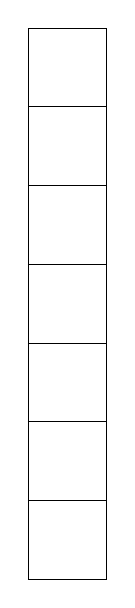
\begin{tikzpicture}
		\draw[step=1cm,black,very thin] (8,-0) grid (9,7);
	\end{tikzpicture}}

%\end{minipage}
%\end{document}
}}\hspace{0.5em}
	\subfloat[After \acrshort{MC} applied]{\scalebox{0.625}{%\end{minipage}
\def\rowperm{{0, 1, 2, 3, 4, 5, 6}}
%\def\colperm{{0, 1, 2, 3, 4, 5, 6}}
\def\colperm{{0, 1, 2, 3, 4, 5, 6}}
%\begin{minipage}{0.55\textwidth}
%\centering
\scalebox{0.7}{\begin{tikzpicture}
	\foreach \x in {0,1}
	\fill[red!65!white] (\colperm[\x]-1,6) rectangle (\colperm[\x],7);  
	\foreach \x in {0,1,2}
	\fill[red!65!white] (\colperm[2+\x]-1,5) rectangle (\colperm[2+\x],6);   
	\foreach \x in {0,1}
	\fill[red!65!white] (\colperm[5+\x]-1,4) rectangle (\colperm[5+\x],5); 

	\node at (\colperm[0]-0.5,6.5) {\Large{1}}; 
	\node at (\colperm[1]-0.5,6.5) {\Large{1}}; 
	\node at (\colperm[2]-0.5,5.5) {\Large{2}}; 
	\node at (\colperm[3]-0.5,5.5) {\Large{2}}; 
	\node at (\colperm[4]-0.5,5.5) {\Large{2}}; 
	\node at (\colperm[5]-0.5,4.5) {\Large{3}}; 
	\node at (\colperm[6]-0.5,4.5) {\Large{3}}; 
	
	\foreach \x in {0,1,2}
	\fill[green!65!white] (\colperm[\x]-1,3) rectangle (\colperm[\x],4);  
	\foreach \x in {0,1,2}
	\fill[green!65!white] (\colperm[3+\x]-1,2) rectangle (\colperm[3+\x],3);   
	\draw[step=1cm,gray,very thin] (-1,-0) grid (6,7);
	\node at (\colperm[0]-0.5,3.5) {\Large{1}}; 
	\node at (\colperm[1]-0.5,3.5) {\Large{1}}; 
	\node at (\colperm[2]-0.5,3.5) {\Large{1}}; 
	\node at (\colperm[3]-0.5,2.5) {\Large{2}}; 
	\node at (\colperm[4]-0.5,2.5) {\Large{2}}; 
	\node at (\colperm[5]-0.5,2.5) {\Large{2}}; 
	
	\foreach \x in {0,1,2}
	\fill[blue!65!white] (\colperm[1+\x]-1,1) rectangle (\colperm[1+\x],2);  
	\foreach \x in {0,1,2}
	\fill[blue!65!white] (\colperm[4+\x]-1,0) rectangle (\colperm[4+\x],1);
	\draw[step=1cm,gray,very thin] (-1,-0) grid (6,7);   
	
	\node at (\colperm[1]-0.5,1.5) {\Large{1}}; 
	\node at (\colperm[2]-0.5,1.5) {\Large{1}}; 
	\node at (\colperm[3]-0.5,1.5) {\Large{1}}; 
	\node at (\colperm[4]-0.5,0.5) {\Large{2}}; 
	\node at (\colperm[5]-0.5,0.5) {\Large{2}}; 
	\node at (\colperm[6]-0.5,0.5) {\Large{2}}; 
	\draw[step=1cm,black,very thin] (-1,-0) grid (6,7);
\end{tikzpicture}}
\hspace{0.3cm}
\scalebox{0.7}{\begin{tikzpicture}
	\foreach \x in {0,1,2,3,4,5,6}
	\fill[red!65!white] (8,\x) rectangle (9,\x+1);  
	\draw[step=1cm,black,very thin] (8,-0) grid (9,7);
	\node at (8.5,6.5-\colperm[0]) {\Large{1}}; 
	\node at (8.5,6.5-\colperm[1]) {\Large{1}}; 
	\node at (8.5,6.5-\colperm[2]) {\Large{2}}; 
	\node at (8.5,6.5-\colperm[3]) {\Large{2}}; 
	\node at (8.5,6.5-\colperm[4]) {\Large{2}}; 
	\node at (8.5,6.5-\colperm[5]) {\Large{3}}; 
	\node at (8.5,6.5-\colperm[6]) {\Large{3}}; 
\end{tikzpicture}}
%\end{minipage}
%\end{document}
}}
	%	\includegraphics[scale=0.6]{pics/alpha_problem/mc_alpha_unsymm_only_red.tex}
	\caption{Illustration of data locality degradation due to \acrshort{MC}.
		Numbers represent thread id}
\end{figure}

\begin{itemize}
	\item Start with MC and ABMC weakness, Spin matrix
	\item Hardware efficiency and performance
	\item Stress on data locality
	\item Optimal permutations
	\item Work on simple data storage format like \acrshort{CRS}
\end{itemize}


\section{RACE method}
\begin{itemize}
	\item The three steps, stress on locality
	\item Recursion very brief and tree
\end{itemize}


\section{Results \& Contribution} \label{sec:results}
\begin{itemize}
	\item Test setup, brief is sufficient
	\item Start with Spin matrix, and little RLM
	\item SymmSpMV performance
\end{itemize}
\subsection{FEAST with RACE}
\begin{itemize}
	\item Briefly describe FEAST
	\item Tell its implemented in MKL, we use Reverse Communication Interface (RCI) of
		\acrshort{MKL} to implement inner linear solver
	\item Tell why we need KACZ -> ill-conditioned linear system, robustness of KACZ -> only potential iterative solver. Tell 99\% of time it uses in this CGMN solver
	\item To our knowledge first implementation that uses iterative inner linear system, which is really inevitable to scale and for large size problems
	\item  Test setup, discrete laplacian, 10 inner eigenvalues, complex numbers 
	\item Comparison with default Pardiso
	\item Discuss on Big O ....
\end{itemize}

\subsection{Acknowledgements}
\begin{itemize}
	\item Thomas Gruber
	\item RRZE and RWTH for providing computations time.
\end{itemize}

\section{Future Work}



\bibliographystyle{ACM-Reference-Format}
\bibliography{RACE_references}

\end{document}
